\documentclass{article}
\usepackage[utf8]{inputenc}
\usepackage{graphicx}
\usepackage{lmodern}
\usepackage[T1]{fontenc}
\usepackage[utf8]{inputenc}
\usepackage[brazilian]{babel}

\title{Projeto para disciplina MAC0350}

\author{
	Gustavo Silva\\
	\texttt{9298260}
	\and
	Leonardo Padilha\\
	\texttt{9298295}
	\and
	Lucas Santos\\
	\texttt{9345064}
	\and
	Marcos Kawakami\\
	\texttt{8041331}
	\and
	Matheus Oliveira\\
	\texttt{8642821}
	\and
	Victor Sena\\
	\texttt{8941317}
}

\date{Outubro de 2017}


\begin{document}

\maketitle

\newpage

\tableofcontents

\newpage

\section{Análise de Requisitos}

	\subsection{Introdução}
	Este sistema tem objetivo de auxiliar o gerenciamento de projetos, incluindo análises de requisitos. Cada projeto será subdividido em atividades, sendo cada atividade relacionada a um requisito do projeto. Ademais, as atividades e projetos estarão associados com um desenvolvedor. Por fim, esse documento tem o objetivo de expor a interação entre os desenvolvedores, os projetos e as atividades tal qual o gerenciamento do projeto como um todo.

	\subsection{Participação de projetos e atividades}
	Todo projeto pode ser criado ou removido por um desenvolvedor. O administrador do projeto é o desenvolvedor que criou o projeto e esse é o único capaz de removê-lo. É importante ressaltar, todavia, que cada projeto pode possuir mais de um desenvolvedor, ainda que apenas um administrador.

	Um projeto possui atividades e cada atividade representa um requisito que estará presente no projeto. Uma atividade deve possuir um ou mais desenvolvedores responsáveis e um desenvolvedor pode ser responsável por várias atividades. Cada atividade possui uma data de início e uma data de finalização e pode ser criada por qualquer desenvolvedor do projeto.

	\subsection{Funcionalidades dos projetos}
	\begin{itemize}
		\item \textbf{Organização das atividades do projeto.} Todo projeto é composto por uma série de atividades que precisam ser cumpridas. Cada atividade possui pelo menos um desenvolvedor associado, que está responsável pela sua entrega.

		\item \textbf{Comunicação entre os desenvolvedores.} Todo projeto possui um fórum de discussão associado. Um fórum de discussão é um conjunto tópicos. Cada tópico deve ser criado por um único desenvolvedor. Um tópico é formado por um conjunto de mensagens ordenadas. Uma mensagem é uma publicação escrita por um desenvolvedor.

		\item \textbf{Controle de datas de entrega das atividades.} Toda atividade possui uma data de início e uma data de entrega associada. Os desenvolvedores podem ter uma visão panorâmica do projeto a partir do cronograma das atividades.
	\end{itemize}


\section{Requisitos de Dados}

	\subsection{Introdução}
	Fazem parte desse sistema as seguintes entidades:
	\begin{itemize}
		\item Desenvolvedor
		\item Projeto
		\item Atividade
		\item Fórum \textit{(de discussão)}
		\item Tópico
		\item Mensagem
	\end{itemize}

	\subsection{Detalhamento das entidades}

		\subsubsection{Desenvolvedor}
		Uma representação de uma pessoa, que trabalha como desenvolvedor, no sistema. As informações a serem registradas são o nome, e-mail (para identificação única e autenticação no sistema), senha para acesso.

		\subsubsection{Projeto}
		Uma representação de um projeto que está sendo ou já foi desenvolvido no sistema. As informações a serem registradas são o nome, uma descrição, uma data de criação e o estado atual do projeto. Cada projeto é univocamente identificado por um atributo-chave inteiro de identificação.

		\subsubsection{Atividade}
		Uma representação de uma ativdade relacionado a um projeto no sistema. As informações que serão guardadas são o nome, uma descrição, data de início, data de término, a qual projeto essa atividade pertence e o estado dessa atividade (se já foi concluída ou não). Cada atividade é representada por um inteiro.

		\subsubsection{Fórum (de discussão)}
		Uma representação de um fórum de discussão de um projeto no sistema. O fórum possui diversos tópicos associados que são criados pelos desenvolvedores. A única informação a ser guardada é a qual projeto o fórum esta associado.

		\subsubsection{Tópico}
		Uma representação de um tópico relacionado a um fórum de discussões. O tópico possui diversas mensagens associadas que são criadas pelos desenvolvedores. As informações a serem registradas são um título, data de criação, qual fórum o tópico e qual desenvolvedor está associado. Cada tópico é univocamente identificado por um atributo-chave inteiro.

		\subsubsection{Mensagem}
		Uma representação de uma mensagem enviada por um desenvolvedor relacionada a um tópico. As informações a serem registradas são o texto, a data de criação e o tópico relacionado. Cada mensagem é identificada univocamente por um número inteiro.

\section{Requisitos Funcionais}

	\subsection{Desenvolvedor}
	Uma pessoa pode se cadastrar no sistema como desenvolvedor;\\
	Um desenvolvedor pode remover sua conta do sistema.

	\subsection{Projeto}
	Um desenvolvedor pode criar vários projetos no sistema;\\
	O desenvolvedor que criou o projeto passará a ser o administrador do mesmo;\\
	O administrador pode adicionar diversos desenvolvedores para participar do projeto;\\
	Os desenvolvedores participantes do projeto podem criar, alterar e remover atividades do projeto;\\
	O administrador pode remover o projeto do sistema.

	\subsection{Atividade}
	Qualquer desenvolvedor participante do projeto pode criar uma atividade;\\
	O desenvolvedor que criou a atividade pode alterâ-la ou removê-la;\\
	O administrador do projeto pode alterar ou remover qualquer atividade do projeto.

	\subsection{Cronograma}
	Um desenvolvedor pode alterar o estado de uma atividade que tenha ele vinculado como responsável;\\
	O administrador do projeto pode alterar o estado de uma atividade relacionado ao projeto.\\

	\subsection{Fórum (de discussão)}
	Um fórum de discussão precisa ser vinculado à um projeto;\\
	Um fórum de discussão é criado automaticamente na criação de um novo projeto;\\
	Quando um projeto é removido, o seu fórum de discussões é removido em cascata;\\

	\subsection{Tópico}
	Um tópico precisa ser vinculado à um fórum de discussões;\\
	Qualquer desenvolvedor associado a um projeto pode criar um tópico no fórum de discussão associado ao projeto;\\
	Um tópico pode ser removido ou alterado apenas pelo seu criador ou pelo administrador do projeto a qual o tópico está indiretamente relacionado (por meio do fórum de discussão).

	\subsection{Mensagem}
	Qualquer desenvolvedor relacionado ao projeto pode criar uma mensagem em qualquer tópico relacionado ao fórum de discussão associado ao projeto;\\
	Uma mensagem pode ser removida pelo criador da mensagem, do tópico associado ou administrador do projeto.


\section{Operações de criação, leitura, atualização e destrução de dados mais frequentes}

	São algumas operações mais frequentes:
	
	\begin{itemize}
		\item Busca por usuário por e-mail e senha, para autenticação;
		\item Busca de projetos por desenvolvedor associado (dado um desenvolvedor fixo), para listagem de projetos do desenvolvedor autenticado;
		\item Listagem de atividades por um projeto, para listagem de atividades de um projeto;
		\item Busca de um fórum de discussão por um projeto, para encontrar o fórum associado;
		\item Listagem de tópicos por um fórum de discussão, para listar os tópicos de um fórum;
		\item Listagem de mensagems por um tópico específico;
		\item Listagem de atividades ainda não concluídas, para construção do cronograma;
		\item Listagem de atividades atrasadas, para definir prioridades no cronograma;
	\end{itemize}


\section{Modelagem Conceitual}

	\subsection{Modelagem ER-X}
	Abaixo segue a modelagem usando o modelo Entidade Relacionamento Extendido do nosso sistema:\\
	\makebox[\textwidth]{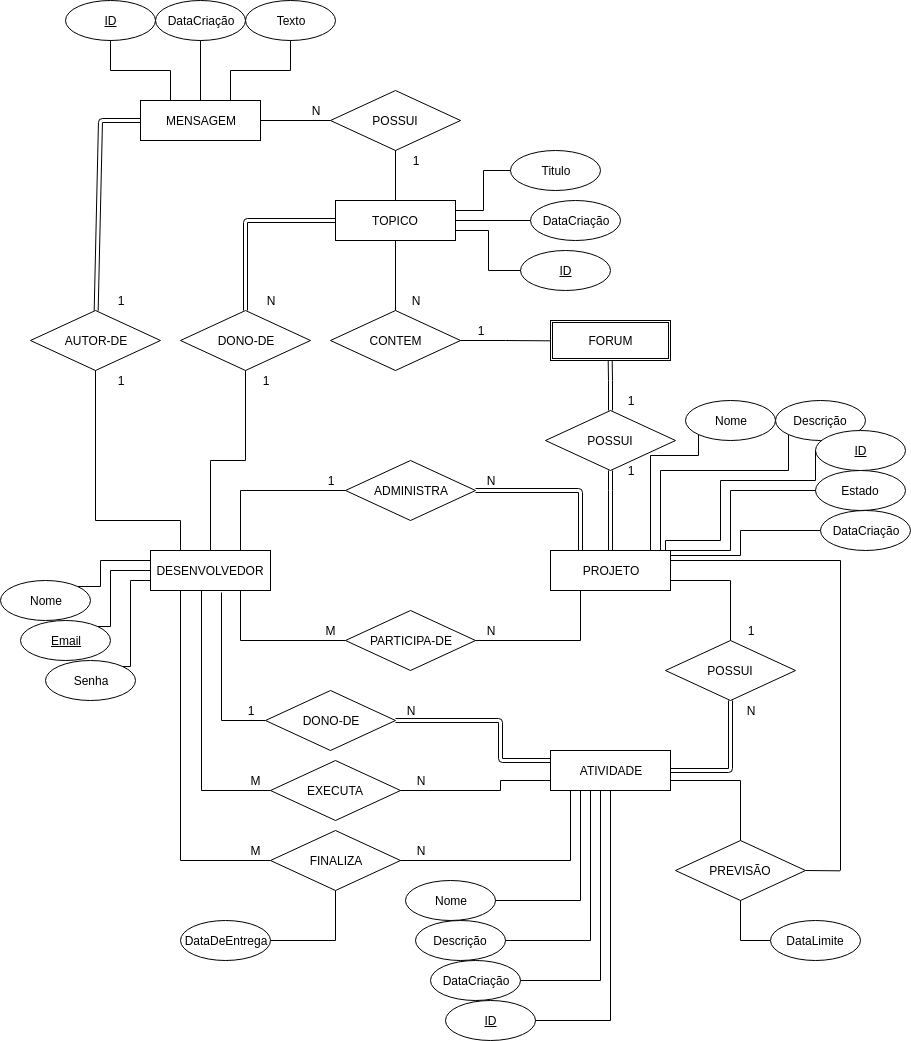
\includegraphics[width=14cm]{img/erx.png}}

	\subsection{Modelagem UML}
	Abaixo segue a modelagem usando o modelo UML do nosso sistema:\\
	\makebox[\textwidth]{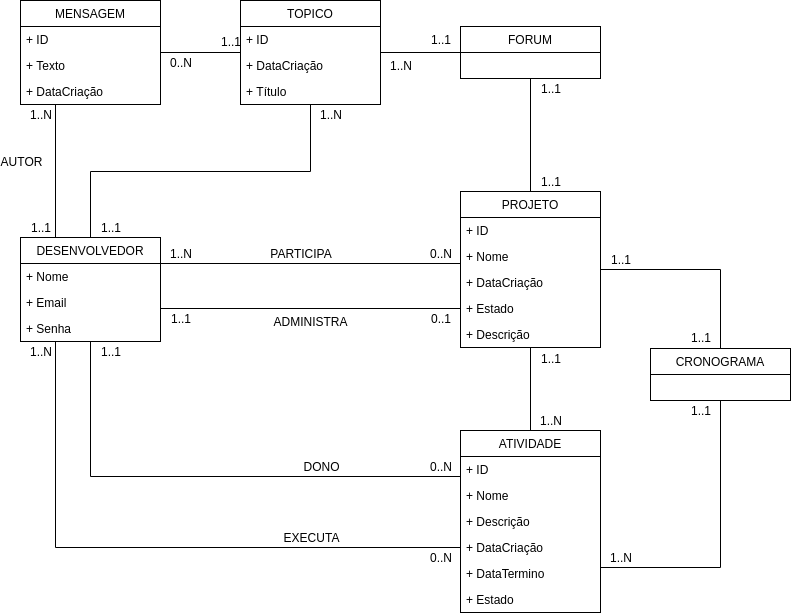
\includegraphics[width=14cm]{img/uml.png}}

	\subsection{Comparação entre ER-X e UML}
	A diferença mais clara entre os modelos é a valorização do relacionamento entre as entidades no primeiro diagrama, enquanto no segundo (UML) existe um foco maior em mostrar as entidades e seus atributos relacionados.\\
	Fica perceptivel, além disso, que o diagrama UML é mais intuitivo quando se trata em compreender as entidades e os atributos. \\
	Entretanto, vale ressaltar que, apesar das diferenças apresentadas na representação, ambas possuem as mesmas \textbf{abstrações dos dados}, modelando os mesmos objetos.

\section{Modelagem Lógica}
	Nossa modelagem lógica usará um \textbf{Modelo Relacional}, dado que nosso SGBD também será relacional. Temos, abaixo, o esquema de todas as relações do nosso sistema:\\
	\makebox[\textwidth]{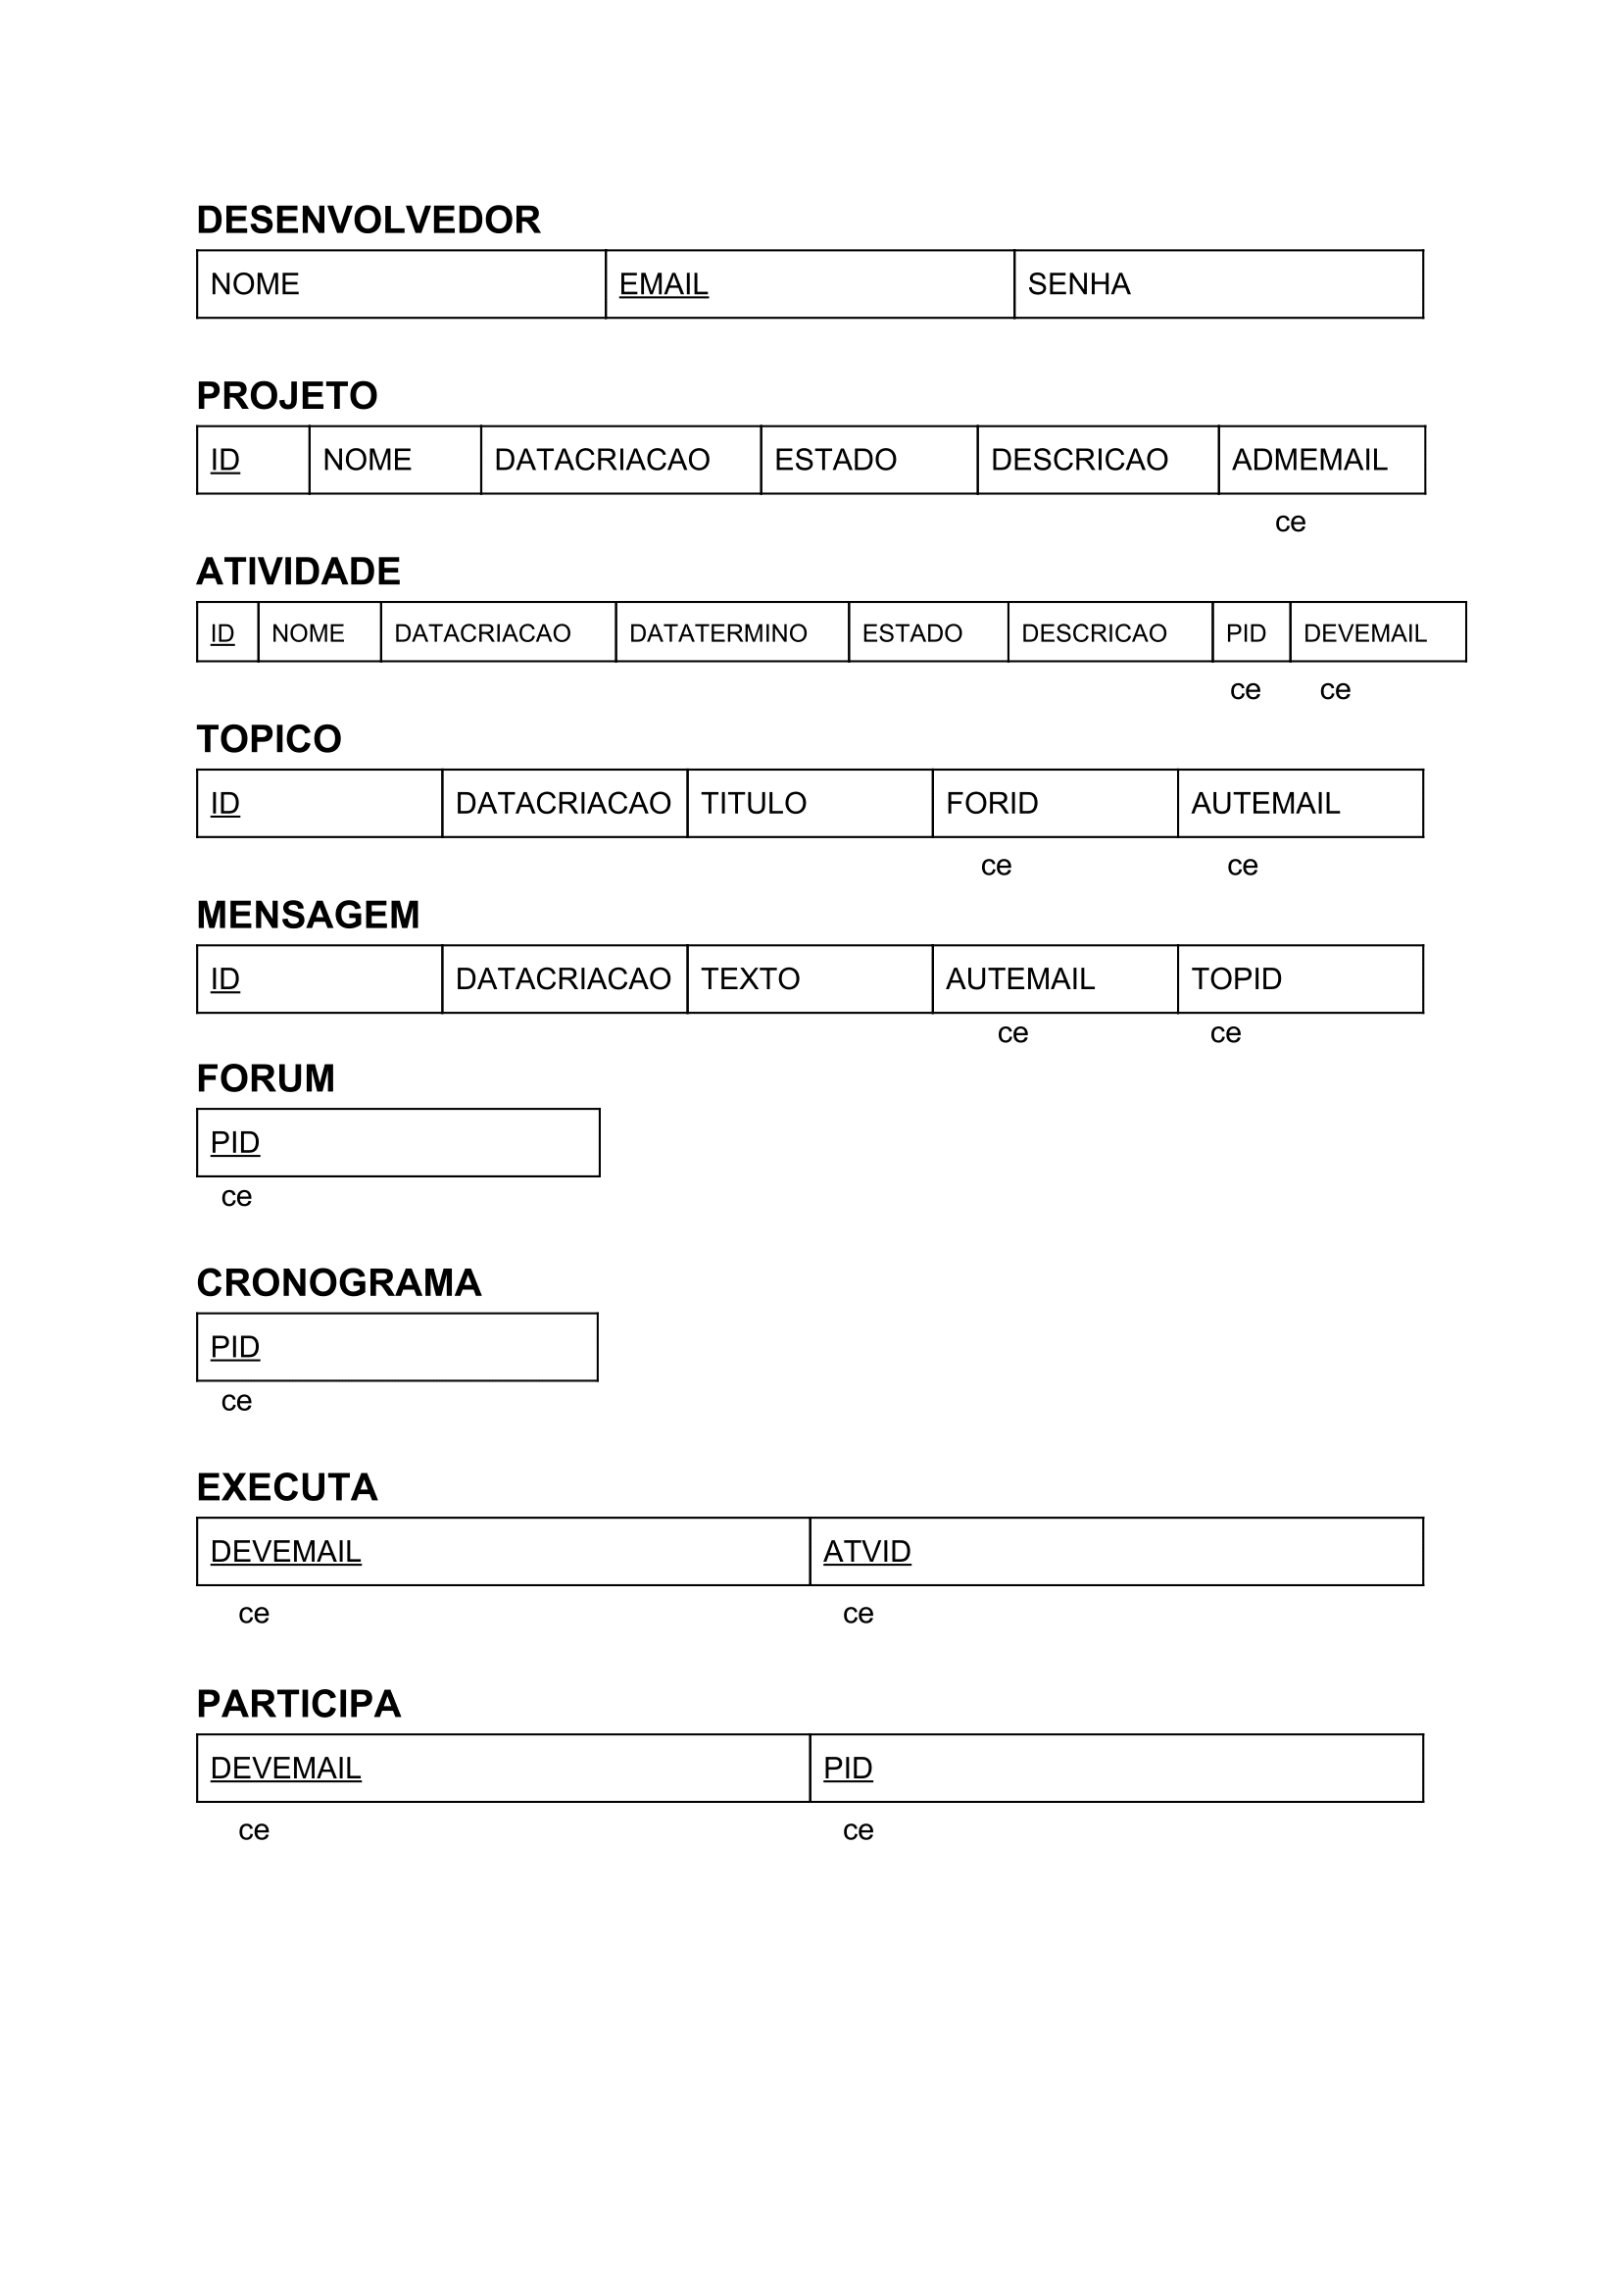
\includegraphics[width=14cm]{img/relacional.png}}


\section{Modelagem Física}
	Para a modelagem física, vamos dividir em duas partes: a primeira será a criação das relações (DDL) e a segunda será o povoamento do banco de dados com nossas informações (DML).
	\subsection{DDL}
		O script de DDL se encontra juntamente com esse documento. Nele, fazemos a criação de todas as relações do sistema, tendo em vista que o SGBD é um PostgreSQL. Diversas restrições de dados podem ser encontradas no script, isso garante que alguns dados sempre estejam presentes nas tuplas.

	\subsection{DML}
		Para a manipulação de dados, criamos um script (que se encontra juntamente com esse documento) que adiciona diversas informações no banco de dados que criamos anteriormente. Além da população, nosso script também realizará algumas consultas ao banco de dados, são elas:
		\begin{itemize}
			\item Obter as atividades do projeto identificado por 1.

			\item Obter o nome dos desenvolvedores que terminaram pelo menos uma atividade.

			\item Obter o nome dos projetos no qual o desenvolvedor cujo email é "green@gmail.com"\\ enviou uma mensagem.

		\end{itemize}


\end{document}
